\chapter{CA-Stream: Attention-based pooling for interpretable image recognition}
\chaptertoc{}
\label{ch:castream}
\section{Introduction}
\label{sec:intro}
%--------------------------------------------------------------------------------------------------
\noindent Another way to approach interpretability can be pointed towards the current advances in recognition 
in general. In particular, with the introduction of the transformer architecture (\cite{vaswani2017attention})
 a switch in the paradigmn occurred where the best performing architectures contain the self-attention 
module as a building block. Moreover with the proposal of the Vision Transformer 
(\cite{dosovitskiy2020image}) transformers were adopted into computer vision, this module gained 
prominence as it allowed models to push the boundaries in existing benchmarks. This led to an 
expansion with models such as Swin-T (\cite{liu2021swin}), LeViT \cite{graham2021levit}. Conversely
hybrid architectures combining ideas from both \gls{cnn} and transformers can be observed 
like Conformer (\cite{peng2021conformer}), Patchconvnet (\cite{touvron2021augmenting}),
while on another hand a modernization of CNNs in the shape of ConvNeXt (\cite{liu2022convnet}) drew 
inspiration from these models, whilst adressing their shortcomings in downstream tasks.\\

\noindent Although these models have pushed visual recognition to new frontiers, their interpretable
 properties still require further exploration, as in one hand conventional interpretability 
methodologies for CNNs do not translate properly into their domain, all the while the explanations 
obtained from these methods (\cite{abnar2020quantifying}) do not appear to have a proper evaluation 
protocol, resulting in research aimed at improved visualizations and their asssesment 
(\cite{chefer2021transformer}).

\noindent In this chapter we study the correlation between CAM and one such attention visualization 
proposal that is the raw attention found in the classification (\cls) token (\cite{devlin2018bert}).
In particular, we note that self attention is defined for all patch tokens including \cls, however 
we can generate cross attention between this token and the feature maps found at any given depth 
of a CNN; this being expressed in via linear combination of feature maps with this token, ultimately 
resembling a class agnostic CAM. As an extension of this, we propose the inclusion of a 
cross-attention module used to train this token as a replacement of GAP (\cite{lin2013network}), 
onto already trained models boosting  both their recognition and interpretable properties.



%quite in great value due to their class agnostic behavior due their class token (\Th{[CLS]}) used for 
%classification(\cite{devlin2018bert}).

%Convolutional neural networks have had tremendous success in computer vision \cite{he2016deep,liu2022convnet} 
%but, due to their complexity, it is still an open problem how to explain or interpret their predictions. 
%The most concrete achievement in this direction is to localize in an image what regions a prediction can be 
%attributed to, by means of \emph{saliency maps}. \emph{Post-hoc} interpretability methods do so without changing 
%the network architecture or training process and \emph{class activation mapping} (CAM)~\cite{zhou2016learning} 
%has been a milestone in their development. CAM-based saliency maps are expressed as a linear combination of 
%feature maps followed by an activation function and it is the definition of weights that determines different 
%methods \cite{DBLP:journals/corr/SelvarajuDVCPB16,DBLP:journals/corr/abs-1710-11063,DBLP:journals/corr/abs-1910-01279}.
%Grad-CAM~\cite{DBLP:journals/corr/SelvarajuDVCPB16}, Grad-CAM++~\cite{DBLP:journals/corr/abs-1710-11063} and ScoreCAM~\cite{DBLP:journals/corr/abs-1910-01279}


%Vision transformers~\cite{dosovitskiy2020image} are now strong competitors of convolutional networks, 
%characterized by global interactions between patch embeddings in the form of \emph{self attention}. 
%Based on a classification (\cls) token, their pooling mechanism allows localization by means of 
%\emph{raw attention} maps. However, these maps are class agnostic, they can be of low quality~\cite{dino} 
%and dedicated interpretability methods are required~\cite{chefer2021transformer}.

%In this work, we make an important connection between CAM and the raw attention map of the \cls token. 
%In particular, self attention is defined on all patch tokens, including \cls. Focusing on the cross attention 
%between \cls and patch token embeddings, this is expressed as a collection of dot product similarities 
%between embeddings, followed by softmax. 
%We show that this collection of similarities is in fact a linear combination of feature maps, where the 
%weights are the elements of the \cls token embedding. Hence, 
%\textbf{the raw attention map of the \cls token has the same form as a class agnostic CAM-based saliency map}.

%In addition, pooling in vision transformers is defined as a weighted average of patch token embeddings, 
%where the weights are given by the raw attention map of the \cls token. This can be seen as reweighting, 
%or soft masking, of the embeddings before \emph{global average pooling} (GAP). By contrast, pooling in 
%convolutional networks is based on GAP only. We thus observe that \textbf{attention-based pooling is a form of masking in the feature space}. Masking, mostly in the input space, is common in interpretability methods~\cite{DBLP:journals/corr/abs-1910-01279} and their evaluation~\cite{DBLP:journals/corr/abs-1710-11063, petsiuk2018rise} to establish that a prediction is indeed due to a certain object of interest.

%Motivated by the above observations, we design an attention-based pooling mechanism as a replacement for 
%GAP in convolutional networks. Since this mechanism has the form of a CAM-based saliency map followed by 
%masking, we aim to study the effect of this network modification in interpreting the network predictions.

%Our pooling mechanism, called \emph{\OURS} (\emph{\Ours}), is implemented as a stream running in parallel 
%with the backbone network. At different stages of the network, it allows interaction between a \cls token 
%and patch embeddings by means of cross attention. The \cls token embedding is initialized as a learnable 
%parameter and, at the output of the stream, provides a global image representation for classification.

%We aim at post-hoc interpretability, therefore we keep the network and classifier frozen while learning 
%the parameters of \Ours. We then obtain CAM-based saliency maps by existing post-hoc methods for both GAP 
%and \Ours and compare their performance in terms of interpretability metrics as well as classification accuracy.

%More specifically, we make the following contributions:
%\begin{enumerate}[itemsep=2pt, parsep=0pt, topsep=3pt]
%    \item We show that attention-based pooling in vision transformers is the same as soft masking by a class agnostic CAM-based saliency map (\autoref{subsec:motiv}).
%    \item We design and inject an attention-based pooling mechanism into convolutional networks to replace GAP and study its effect on post-hoc interpretability (\autoref{subsec:CA-base}). This is a modification of the network but not of its training process.
%    \item We show that this mechanism helps explain a trained network by improving the performance of existing post-hoc interpretability methods as well as providing a class agnostic raw attention map (\autoref{sec:exp}).
%\end{enumerate}

%Convolutional neural networks have had tremendous success in computer vision ~\cite{he2016deep,liu2022convnet} but, due
to their complexity, it is still an open problem how to explain or interpret their predictions. The most concrete
achievement in this direction is to localize in an image what regions a prediction can be attributed to, by means of
\emph{saliency maps}. \emph{Post-hoc} interpretability methods do so without changing the network architecture or
training process and \emph{class activation mapping} (CAM)~\cite{zhou2016learning} has been a milestone in their
development. CAM-based saliency maps are expressed as a linear combination of feature maps followed by an activation
function and it is the definition of weights that determines different methods
\cite{DBLP:journals/corr/SelvarajuDVCPB16,DBLP:journals/corr/abs-1710-11063,DBLP:journals/corr/abs-1910-01279}.
%Grad-CAM~\cite{DBLP:journals/corr/SelvarajuDVCPB16}, Grad-CAM++~\cite{DBLP:journals/corr/abs-1710-11063} and
%ScoreCAM~\cite{DBLP:journals/corr/abs-1910-01279}


Vision transformers~\cite{dosovitskiy2020image} are now strong competitors of convolutional networks, characterized by
global interactions between patch embeddings in the form of \emph{self attention}.
Based on a classification (\cls) token, their pooling mechanism allows localization by means of \emph{raw attention}
maps. However, these maps are class agnostic, they can be of low quality~\cite{dino} and dedicated interpretability
methods are required~\cite{chefer2021transformer}.

In this work, we make an important connection between CAM and the raw attention map of the \cls token.
In particular, self attention is defined on all patch tokens, including \cls. Focusing on the cross attention between
\cls and patch token embeddings, this is expressed as a collection of dot product similarities between embeddings,
followed by softmax.
We show that this collection of similarities is in fact a linear combination of feature maps, where the weights are the
elements of the \cls token embedding. Hence, \textbf{the raw attention map of the \cls token has the same form as a
class agnostic CAM-based saliency map}.

In addition, pooling in vision transformers is defined as a weighted average of patch token embeddings, where the
weights are given by the raw attention map of the \cls token. This can be seen as reweighting, or soft masking, of the
embeddings before \emph{global average pooling} (GAP). By contrast, pooling in convolutional networks is based on GAP
only. We thus observe that \textbf{attention-based pooling is a form of masking in the feature space}. Masking, mostly
in the input space, is common in interpretability methods~\cite{DBLP:journals/corr/abs-1910-01279} and their
evaluation~\cite{DBLP:journals/corr/abs-1710-11063, petsiuk2018rise} to establish that a prediction is indeed due to a
certain object of interest.

Motivated by the above observations, we design an attention-based pooling mechanism as a replacement for GAP in
convolutional networks. Since this mechanism has the form of a CAM-based saliency map followed by masking, we aim to
study the effect of this network modification in interpreting the network predictions.

Our pooling mechanism, called \emph{\OURS} (\emph{\Ours}), is implemented as a stream running in parallel with the
backbone network. At different stages of the network, it allows interaction between a \cls token and patch embeddings by
means of cross attention. The \cls token embedding is initialized as a learnable parameter and, at the output of the
stream, provides a global image representation for classification.

We aim at post-hoc interpretability, therefore we keep the network and classifier frozen while learning the parameters
of \Ours. We then obtain CAM-based saliency maps by existing post-hoc methods for both GAP and \Ours and compare their
performance in terms of interpretability metrics as well as classification accuracy.


\section {Cross Attention}
\label{sec:ca_defn}

\newpage
%--------------------------------------------------------------------------------------------------
\section{Cross Attention Stream}
\begin{figure*}[t]
    \centering
    \begin{tikzpicture}[
        font={\footnotesize},
        trap/.style={trapezium, rotate=-90,trapezium angle=75},
    ]
        %% CNN branch
        \node(input) at (-5.5, 0) {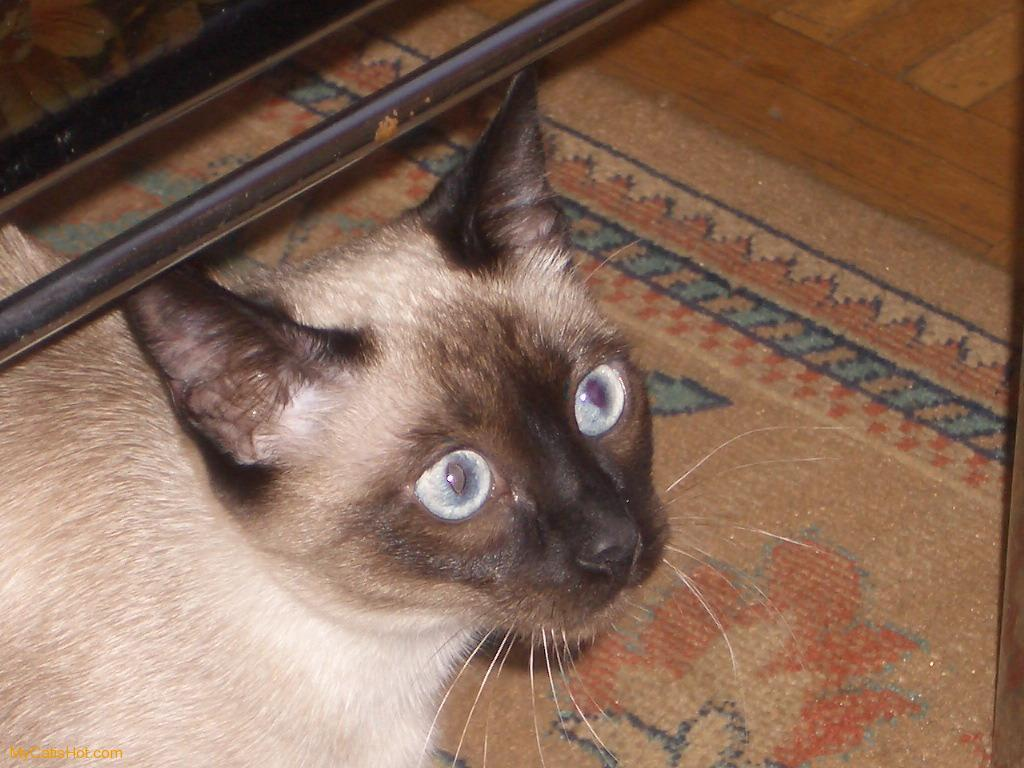
\includegraphics[width=.1\textwidth]{Images/Method/input.jpg}};
        \node[above] at (input.north) {Input image $\vx$};
        \node[draw, trap] (res0) at (-3.5,0) {\rotatebox{90}{\parbox{1.0cm}{\centering{Res-0}}}};
        \node[draw, trap] (res1) at (-1.5,0) {\rotatebox{90}{\parbox{1.0cm}{\centering{Res-1}}}};
        \node[draw, trap] (res2) at (0.5,0) {\rotatebox{90}{\parbox{1.0cm}{\centering{Res-2}}}};
        \node[draw, trap] (res3) at (2.5,0) {\rotatebox{90}{\parbox{1.0cm}{\centering{Res-3}}}};
        \node[draw, trap] (res4) at (4.5,0) {\rotatebox{90}{\parbox{1.0cm}{\centering{Res-4}}}};
        \node[](empt1) at (6.75, 0){};
        \node[draw, rotate=90, align=center] (class) at (7.5,0) {Classifier};
        \node(logit) at (8.25, 0) {$\vy$};
        %%% CLS stream
        \node[](clsin) at (-4, -1.5) {{$\vq_0$}};
        \node[draw](CA0) at (-2.5, -1.5) {{CA-0}};
        \node[draw](CA1) at (-0.5, -1.5) {{CA-1}};
        \node[draw](CA2) at (1.5, -1.5)  {{CA-2}};
        \node[draw](CA3) at (3.5, -1.5)  {{CA-3}};
        \node[draw](CA4) at (5.5, -1.5)  {{CA-4}};
    
        %% CNN backbone
        \node(empt0) at (-4.65, 0) {};
        \draw[->] (empt0.center) -- node {} (res0);
        \draw[->] (res0) -- node[above] {$F_0$} (res1);
        \draw[->] (res1) -- node[above] {$F_1$} (res2);
        \draw[->] (res2) -- node[above] {$F_2$} (res3);
        \draw[->] (res3) -- node[above] {$F_3$} (res4);
        \draw[->, blue, dashed] (res4) -- node {\blue{\normalsize//}} (class);
        \node[](GAP) at (6.25,0.25) {\blue{$\gap$}};
        \draw[->] (class) -- node {} (logit);
        %% CLS Stream
        \draw[->] (clsin) -- node {} (CA0);
        \draw[dashed, ->] (res0.north) -|node {} (CA0);
        \draw[->] (CA0) -- node[above] {$\vq_1$} (CA1);
        \draw[dashed, ->] (res1.north) -|node {} (CA1);
        \draw[->] (CA1) -- node[above] {$\vq_2$} (CA2);
        \draw[dashed, ->] (res2.north) -|node {} (CA2);
        \draw[->] (CA2) -- node[above] {$\vq_3$} (CA3);
        \draw[dashed, ->] (res3.north) -|node {} (CA3);
        \draw[->] (CA3) -- node[above] {$\vq_4$} (CA4);
        \draw[dashed, ->] (res4.north) -|node[above] {$F_4$} (CA4);
        \draw[-] (CA4.east) -| node[right] {$\vq_5$} (empt1.center);
        \draw[->] (empt1.center) -- node {} (class);
    \end{tikzpicture}
    \vspace{3pt}
    \caption{\emph{\OURS (\Ours) applied to ResNet-based architectures.} Given a network $f$, we replace global average pooling (\gap) by a learned, attention-based pooling mechanism implemented as a stream in parallel to $f$. The feature tensor $F_\ell \in \real^{p_\ell \times d_\ell}$ (\emph{key}) obtained by stage Res-$\ell$ of $f$ interacts with a \cls token (\emph{query}) embedding $\vq_\ell \in \real^{d_\ell}$ in block CA-$\ell$, which contains cross attention~\eq{CA} followed by a linear projection~\eq{qk-layer} to adapt to the dimension of $F_{\ell+1}$. Here, $p_\ell$ is the number of patches (spatial resolution) and $d_\ell$ the embedding dimension. The query is initialized by a learnable parameter $\vq_0 \in \real^{d_0}$, while the output $\vq_5$ of the last cross attention block is used as a global image representation into the classifier. The network and classifier are pretrained and kept frozen while the parameters of \Ours are learned. At inference, we use existing post-hoc interpretability methods like Grad-CAM~\citep{DBLP:journals/corr/SelvarajuDVCPB16} to obtain saliency maps for both the baseline \gap and our \Ours. We compare interpretability metrics as well as accuracy.}
    \label{fig:fig_method}
    \end{figure*}
    
\label{sec:ca_design}
Motivated by the observations above, we design a \emph{\OURS} (\emph{\Ours}) in parallel to any 
network. It takes input features at key locations of the network and uses cross attention to build 
a global image representation and replace $\gap$ before the classifier. An example is shown in 
\autoref{fig:fig_method}, applied to a ResNet-based architecture.

\paragraph{Architecture}
More formally, given a network $f$, we consider points between blocks of $f$ where critical 
operations take place, such as change of spatial resolution or embedding dimension, \eg between 
stages for ResNet. We decompose $f$ at these points as
\begin{equation}
	f = g \circ \gap \circ f_L \circ \dots \circ f_0
\label{eq:f-decomp}
\end{equation}
such that features $F_\ell \in \real^{p_\ell \times d_\ell}$ of layer (stage) $\ell$ are 
initialized as $F_{-1} = \vx$ and updated according to

\begin{equation}
	F_\ell = f_\ell(F_{\ell-1})
\label{eq:f-layer}
\end{equation}
for $0 \le \ell \le L$. The last layer features $F_L$ are followed by \gap and $g: \real^{d_L} \to 
\real^C$ is the classifier, mapping to the logit vector $\vy$. As in ~\eq{sal}, 
$p_\ell$ is the number of patch tokens and $d_\ell$ the embedding dimension of stage $\ell$.

In parallel, we initialize a classification token embedding as a learnable parameter $\vq_0 \in 
\real^{d_0}$ and we build a sequence of updated embeddings $\vq_\ell \in \real^{d_\ell}$ along a 
stream that interacts with $F_\ell$ at each stage $\ell$. Referring to the global representation 
$\vq_\ell$ as \emph{query} or \cls and to the local image features $F_\ell$ as \emph{key} or patch 
embeddings, the interaction consists of cross attention followed by a linear projection $W_\ell \in 
\real^{d_{\ell+1} \times d_\ell}$ to account for changes of embedding dimension between the 
corresponding stages of $f$:

\begin{equation}
	\vq_{\ell+1} = W_\ell \cdot \ca_\ell(\vq_\ell, F_\ell),
\label{eq:qk-layer}
\end{equation}
for $0 \le \ell \le L$, where $\ca_\ell$ is defined as in~\eq{CA}. 
% Because of linearity, projection $W_\ell$ is the same as a value projection.

Image features $F_0, \dots, F_L$ do not change by injecting our \Ours into network $f$. However, 
the final global image representation and hence the prediction do change. In particular, at the 
last stage $L$, $\vq_{L+1}$ is used as a global image representation for classification, 
replacing \gap over $F_L$. The final prediction is $g(\vq_{L+1}) \in \real^C$. Unlike \gap, the 
weights of different image patches in the linear combination are non-uniform, enhancing the 
contribution of relevant patches in the prediction.

%--------------------------------------------------------------------------------------------------
\paragraph{Training}

In this sense, the network $f$ is pretrained and remains frozen while we learn the parameters of 
our \Ours on the same training set as one used to train $f$. The classifier is kept frozen too. 
Referring to~\eq{f-decomp}, $f_0, \dots, f_L$ and $g$ are fixed, while \gap is replaced by learned 
weighted averaging, with the weights obtained by the \Ours.

\paragraph{Inference}
As it stands, \Ours is not an interpretability method, but rather a modification of the baseline 
architecture, \ie, an attention-based pooling mechanism that replaces \gap to enhance the 
contribution of relevant image regions in the prediction. We are interested in investigating the 
interpretability properties of this modification. We therefore employ existing post-hoc, CAM-based 
interpretability methods to generate saliency maps with both baseline \gap and \Ours. We then 
compare interpretability metrics as well as classification accuracy.
\newpage
%--------------------------------------------------------------------------------------------------
\section{Qualitative Results}
\label{sec:ca_qual}
\subsection{Qualitative evaluation}
\label{subsec:vinspection}    
We show saliency maps obtained by different interpretability methods using either \gap or \Ours, as 
well as the class-agnostic raw attention coming from our \Ours, see \autoref{fig:compmethods}.\\
%--------------------------------------------------------------------------------------------------
\begin{figure}[H]
    \scriptsize
    \centering
    \setlength{\tabcolsep}{1.5pt}
    % \resizebox{\textwidth}{!}{%
    \begin{tabular}{ccccccccc}
        {}&\multirow{2}{*}{Input image}&\multirow{2}{*}{Raw Attention}&\multicolumn{2}{c}{Grad-CAM}&\multicolumn{2}{c}{Grad-CAM++}&\multicolumn{1}{c}{Score-CAM}\\
        {}&{}&{}&GAP&\Ours&GAP&\Ours&GAP&\Ours\\   
        {\rotatebox{90}{\tiny Envelope}}&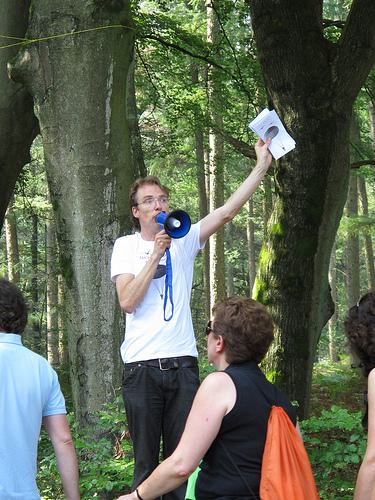
\includegraphics[width=0.11\textwidth]{fig/castream/images/Comparable/figure1_similarities/original/23541.jpeg}&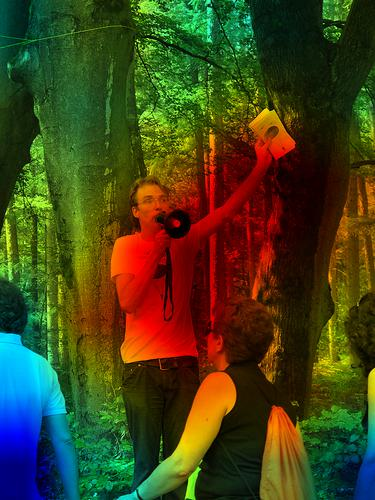
\includegraphics[width=0.11\textwidth]{fig/castream/images/Comparable/figure1_similarities/raw_att/23541.jpeg}&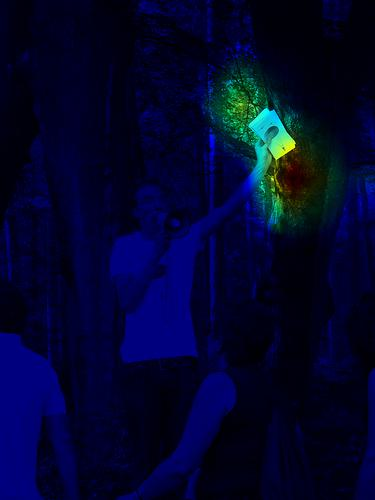
\includegraphics[width=0.11\textwidth]{fig/castream/images/Comparable/figure1_similarities/shelf_gradcam/23541.jpeg}&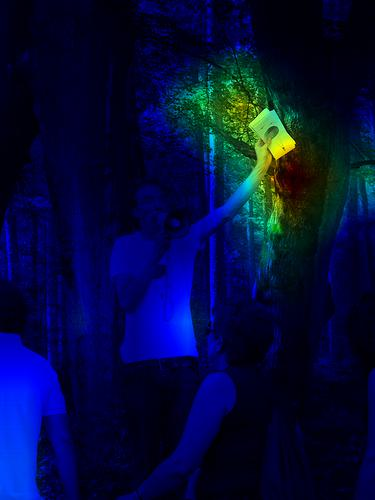
\includegraphics[width=0.11\textwidth]{fig/castream/images/Comparable/figure1_similarities/gradcam/23541.jpeg}&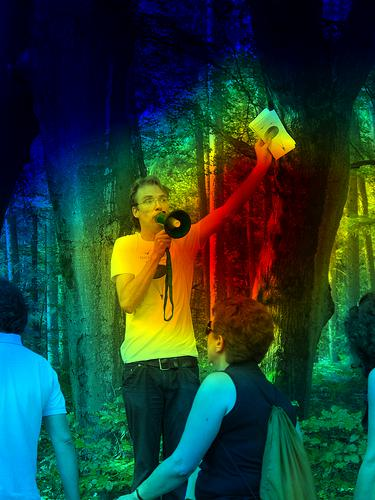
\includegraphics[width=0.11\textwidth]{fig/castream/images/Comparable/figure1_similarities/shelf_gradcampp/23541.jpeg}&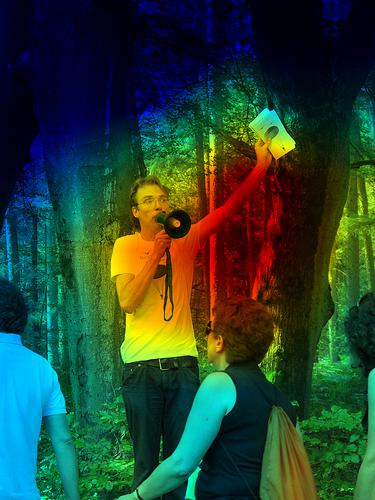
\includegraphics[width=0.11\textwidth]{fig/castream/images/Comparable/figure1_similarities/gradcampp/23541.jpeg}&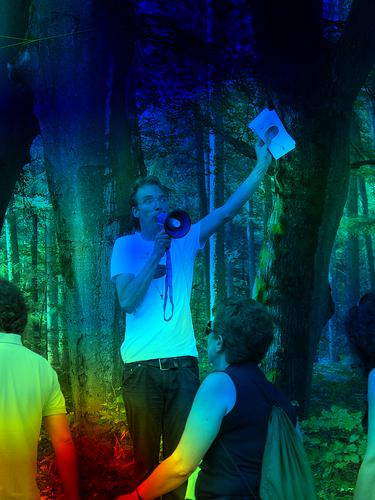
\includegraphics[width=0.11\textwidth]{fig/castream/images/Comparable/figure1_similarities/scorecam/23541.jpeg}&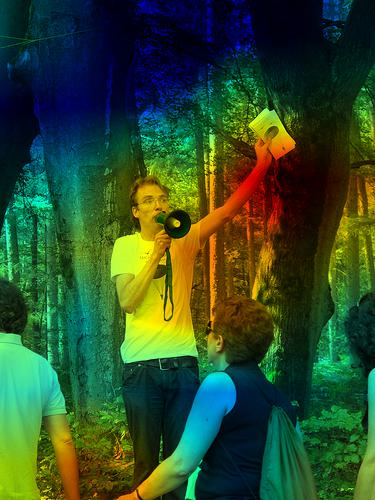
\includegraphics[width=0.11\textwidth]{fig/castream/images/Comparable/figure1_similarities/shelf_scorecam/23541.jpeg}\\
        {\rotatebox{90}{\tiny Groom}}&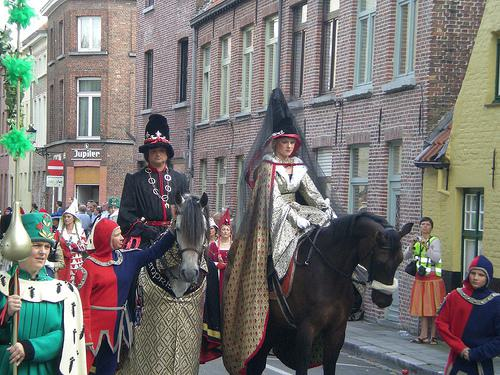
\includegraphics[width=0.11\textwidth]{fig/castream/images/Comparable/figure1_similarities/original/9602.jpeg}&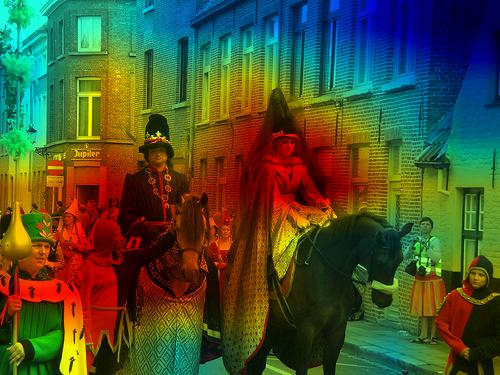
\includegraphics[width=0.11\textwidth]{fig/castream/images/Comparable/figure1_similarities/raw_att/9602.jpeg}&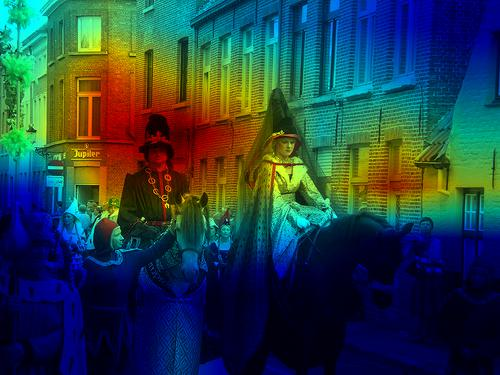
\includegraphics[width=0.11\textwidth]{fig/castream/images/Comparable/figure1_similarities/shelf_gradcam/9602.jpeg}&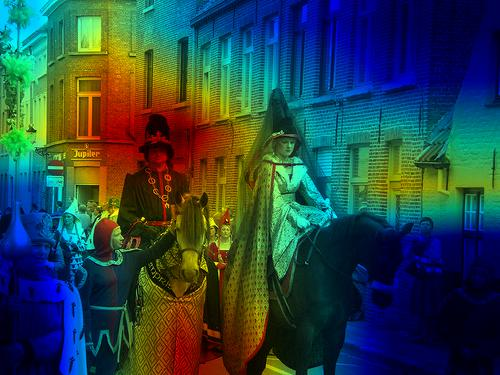
\includegraphics[width=0.11\textwidth]{fig/castream/images/Comparable/figure1_similarities/gradcam/9602.jpeg}&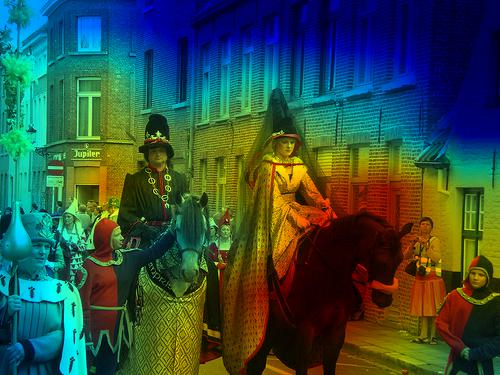
\includegraphics[width=0.11\textwidth]{fig/castream/images/Comparable/figure1_similarities/shelf_gradcampp/9602.jpeg}&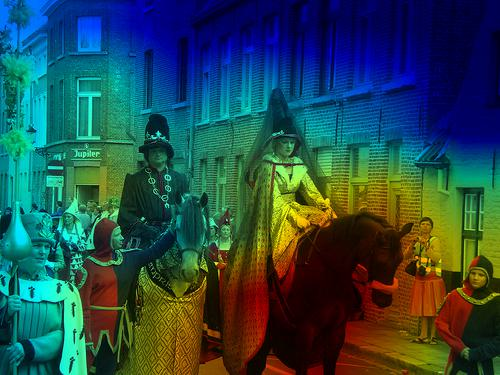
\includegraphics[width=0.11\textwidth]{fig/castream/images/Comparable/figure1_similarities/gradcampp/9602.jpeg}&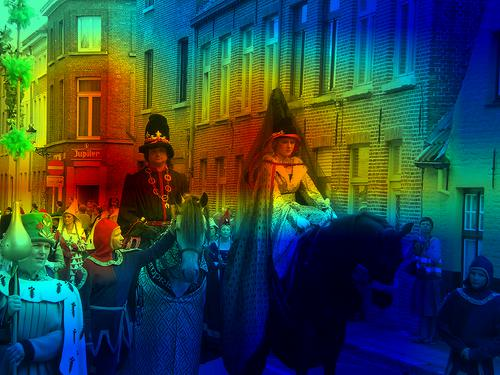
\includegraphics[width=0.11\textwidth]{fig/castream/images/Comparable/figure1_similarities/scorecam/9602.jpeg}&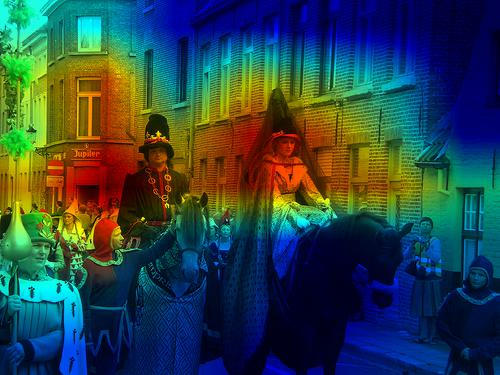
\includegraphics[width=0.11\textwidth]{fig/castream/images/Comparable/figure1_similarities/shelf_scorecam/9602.jpeg}\\    
        {\rotatebox{90}{\tiny Nematode}}&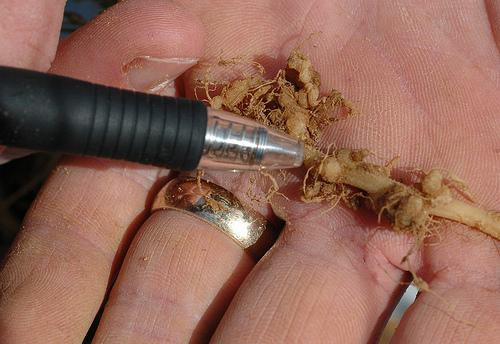
\includegraphics[width=0.11\textwidth]{fig/castream/images/Comparable/figure1_similarities/original/12414.jpeg}&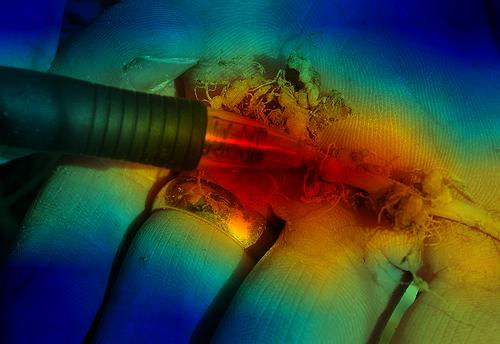
\includegraphics[width=0.11\textwidth]{fig/castream/images/Comparable/figure1_similarities/raw_att/12414.jpeg}&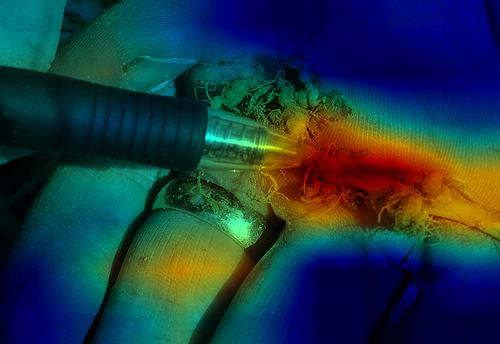
\includegraphics[width=0.11\textwidth]{fig/castream/images/Comparable/figure1_similarities/shelf_gradcam/12414.jpeg}&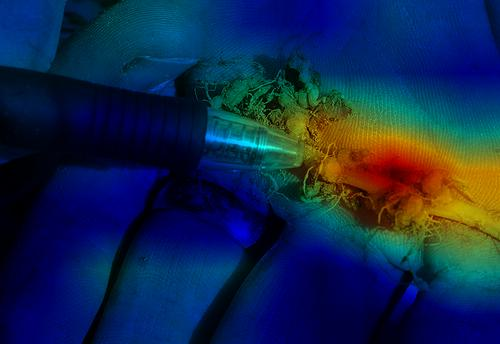
\includegraphics[width=0.11\textwidth]{fig/castream/images/Comparable/figure1_similarities/gradcam/12414.jpeg}&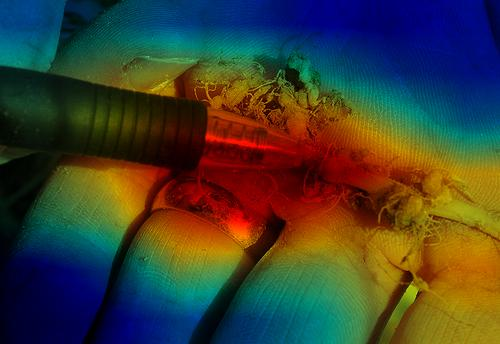
\includegraphics[width=0.11\textwidth]{fig/castream/images/Comparable/figure1_similarities/shelf_gradcampp/12414.jpeg}&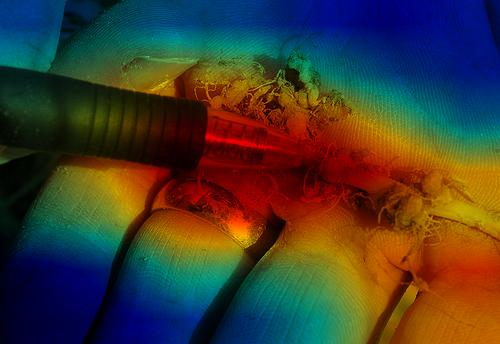
\includegraphics[width=0.11\textwidth]{fig/castream/images/Comparable/figure1_similarities/gradcampp/12414.jpeg}&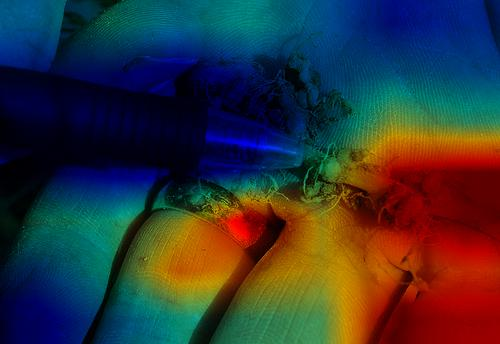
\includegraphics[width=0.11\textwidth]{fig/castream/images/Comparable/figure1_similarities/scorecam/12414.jpeg}&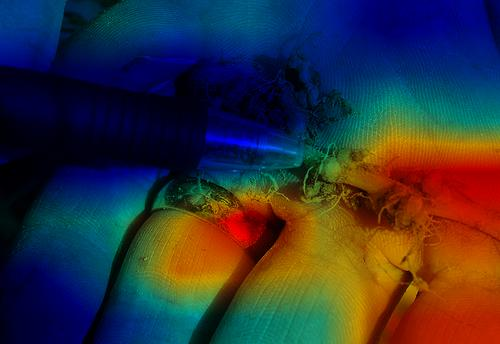
\includegraphics[width=0.11\textwidth]{fig/castream/images/Comparable/figure1_similarities/shelf_scorecam/12414.jpeg}\\
        {\rotatebox{90}{\tiny CRT screen}}&\multicolumn{1}{c}{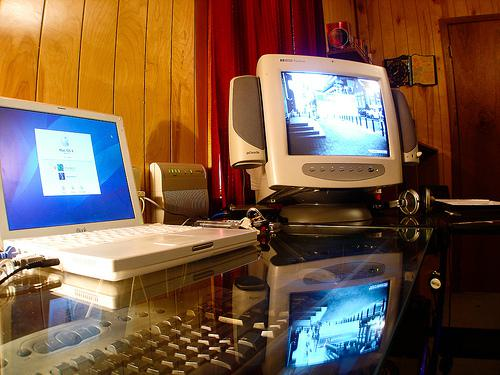
\includegraphics[width=0.11\textwidth]{fig/castream/images/Comparable/figure1/original/43057.jpeg}}&\multicolumn{1}{c}{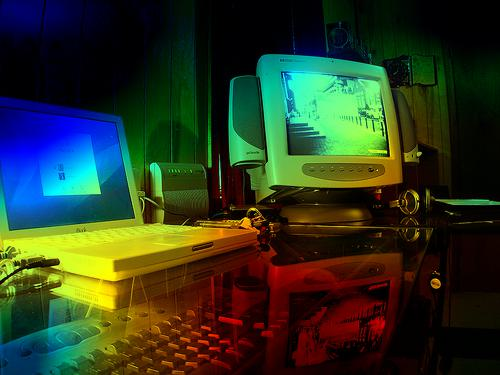
\includegraphics[width=0.11\textwidth]{fig/castream/images/Comparable/figure1/raw_att/43057.jpeg}}&\multicolumn{1}{c}{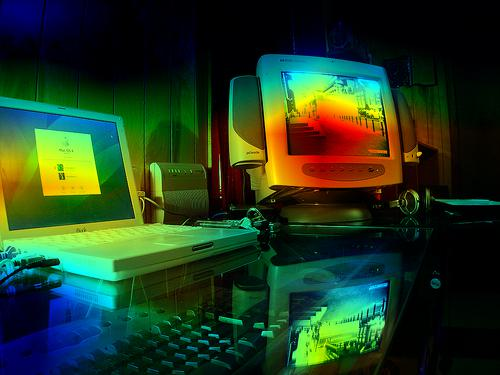
\includegraphics[width=0.11\textwidth]{fig/castream/images/Comparable/figure1/shelf_gradcam/43057.jpeg}}&\multicolumn{1}{c}{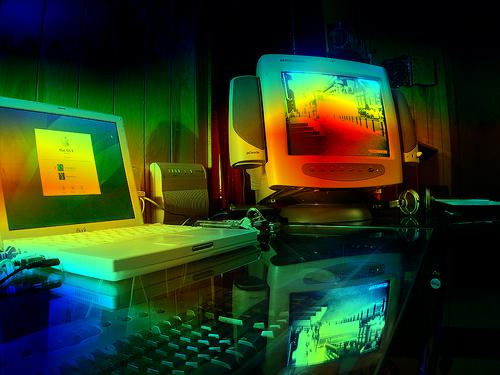
\includegraphics[width=0.11\textwidth]{fig/castream/images/Comparable/figure1/gradcam/43057.jpeg}}&\multicolumn{1}{c}{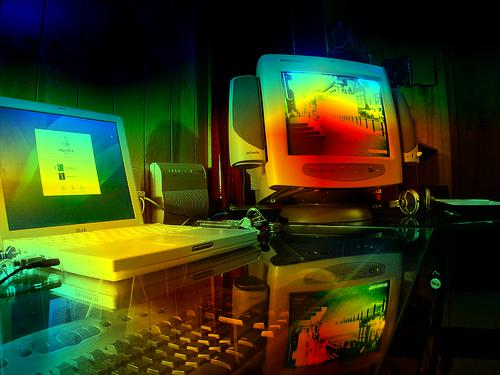
\includegraphics[width=0.11\textwidth]{fig/castream/images/Comparable/figure1/shelf_gradcampp/43057.jpeg}}&\multicolumn{1}{c}{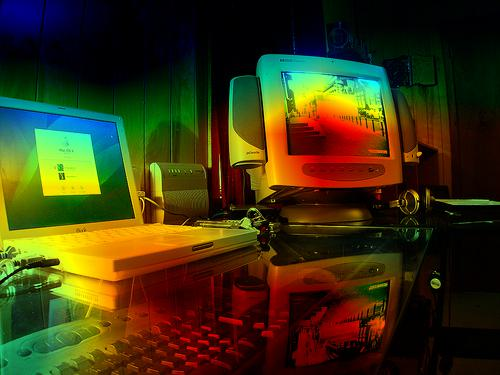
\includegraphics[width=0.11\textwidth]{fig/castream/images/Comparable/figure1/gradcampp/43057.jpeg}}&\multicolumn{1}{c}{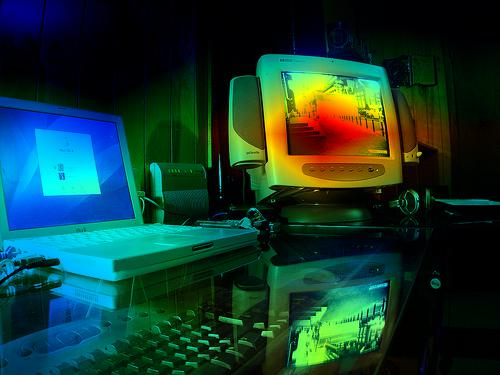
\includegraphics[width=0.11\textwidth]{fig/castream/images/Comparable/figure1/shelf_scorecam/43057.jpeg}}&\multicolumn{1}{c}{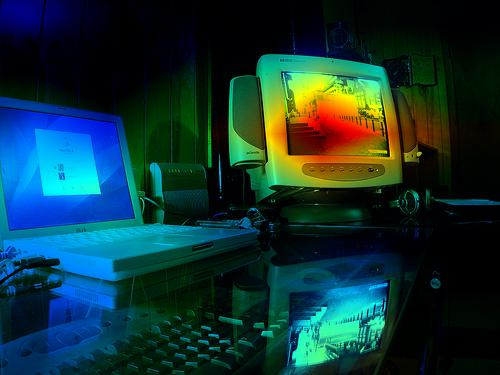
\includegraphics[width=0.11\textwidth]{fig/castream/images/Comparable/figure1/scorecam/43057.jpeg}}\\ % Checked     
        {\rotatebox{90}{\tiny Snowboard}}&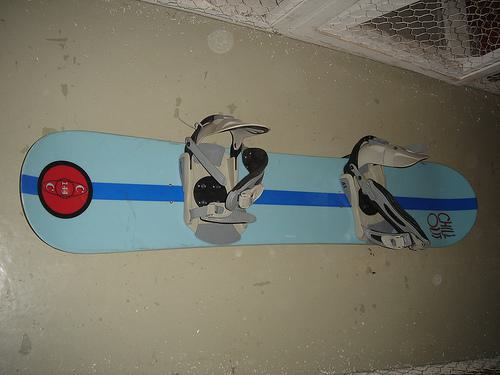
\includegraphics[width=0.11\textwidth]{fig/castream/images/Comparable/figure1_similarities/original/11376.jpeg}&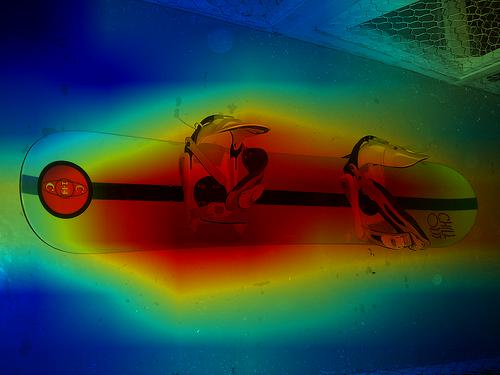
\includegraphics[width=0.11\textwidth]{fig/castream/images/Comparable/figure1_similarities/raw_att/11376.jpeg}&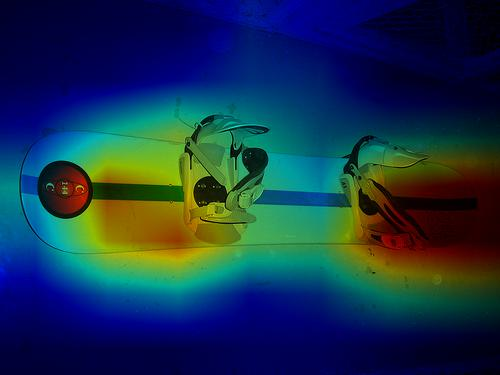
\includegraphics[width=0.11\textwidth]{fig/castream/images/Comparable/figure1_similarities/shelf_gradcam/11376.jpeg}&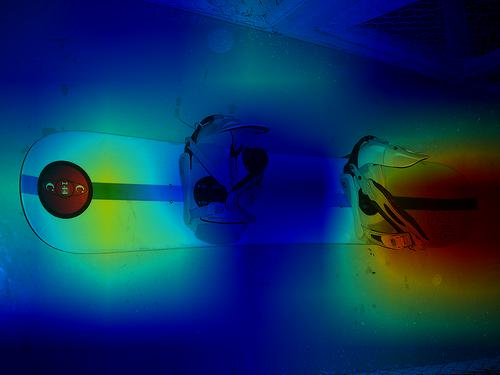
\includegraphics[width=0.11\textwidth]{fig/castream/images/Comparable/figure1_similarities/gradcam/11376.jpeg}&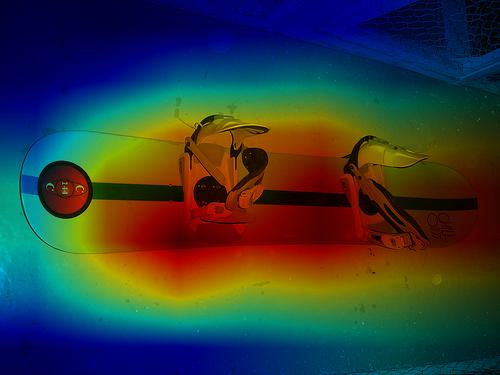
\includegraphics[width=0.11\textwidth]{fig/castream/images/Comparable/figure1_similarities/shelf_gradcampp/11376.jpeg}&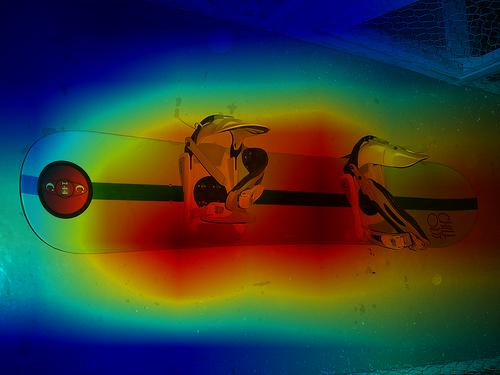
\includegraphics[width=0.11\textwidth]{fig/castream/images/Comparable/figure1_similarities/gradcampp/11376.jpeg}&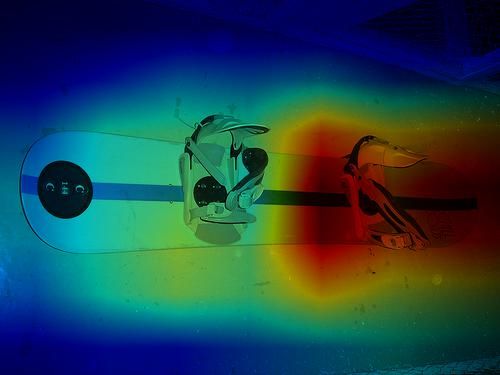
\includegraphics[width=0.11\textwidth]{fig/castream/images/Comparable/figure1_similarities/scorecam/11376.jpeg}&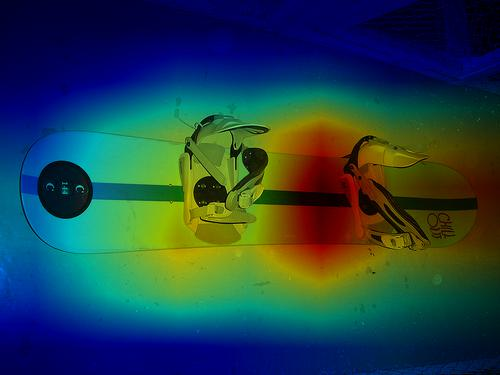
\includegraphics[width=0.11\textwidth]{fig/castream/images/Comparable/figure1_similarities/shelf_scorecam/11376.jpeg}\\   
    \end{tabular}
    % }
    \vspace{3pt}
    \caption{\textbf{Comparison of saliency maps} generated by different CAM-based methods, using GAP and our \Ours, on ImageNet images. The raw attention is the one used for pooling by \Ours.}
    \label{fig:compmethods}
    \end{figure}

We observe that the raw attention focuses on objects of interest in the images. 
In general, saliency maps obtained with \Ours are similar but tend to cover larger regions of the 
object or more instances compared with \gap.\\
\begin{figure}[t]
\scriptsize
\centering
\setlength{\tabcolsep}{1.3pt}
%    \resizebox{\columnwidth}{!}{%
     \begin{tabular}{cccccccc}
           \mc{2}{Corridor}&\mc{2}{Greenhouse}&\mc{2}{Pool Inside}&\mc{2}{Wine Cellar}\\
           Input image&Raw Attention&Input image&Raw Attention&Input image&Raw Attention&Input image&Raw Attention\\
           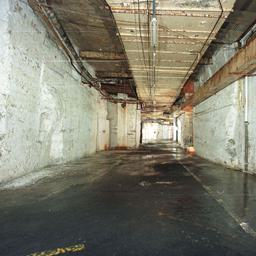
\includegraphics[width=0.12\textwidth,height=0.08\textwidth]{fig/castream/images/Outdataset/Corridor/Original/c1.jpg}&
           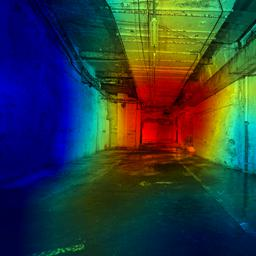
\includegraphics[width=0.12\textwidth,height=0.08\textwidth]{fig/castream/images/Outdataset/Corridor/Attention/c1.jpg}&
           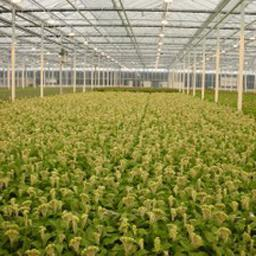
\includegraphics[width=0.12\textwidth,height=0.08\textwidth]{fig/castream/images/Outdataset/Greenhouse/Original/celosie_02.jpg}&
           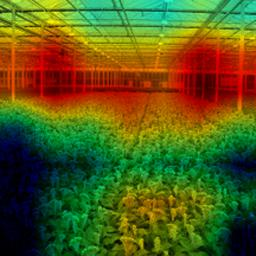
\includegraphics[width=0.12\textwidth,height=0.08\textwidth]{fig/castream/images/Outdataset/Greenhouse/Attention/celosie_02.jpg}&
           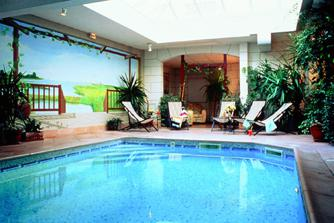
\includegraphics[width=0.12\textwidth,height=0.08\textwidth]{fig/castream/images/Outdataset/Poolinside/Original/003_1b.jpg}&
           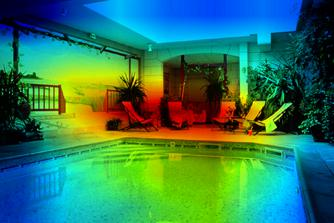
\includegraphics[width=0.12\textwidth,height=0.08\textwidth]{fig/castream/images/Outdataset/Poolinside/Attention/003_1b.jpg}&
           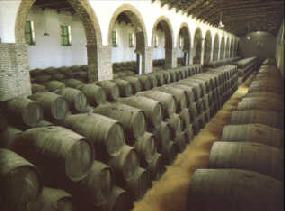
\includegraphics[width=0.12\textwidth,height=0.08\textwidth]{fig/castream/images/Outdataset/WineCellar/Original/bodega2.jpg}&
           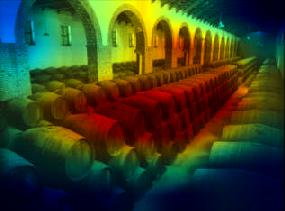
\includegraphics[width=0.12\textwidth,height=0.08\textwidth]{fig/castream/images/Outdataset/WineCellar/Attention/bodega2.jpg}\\
           
           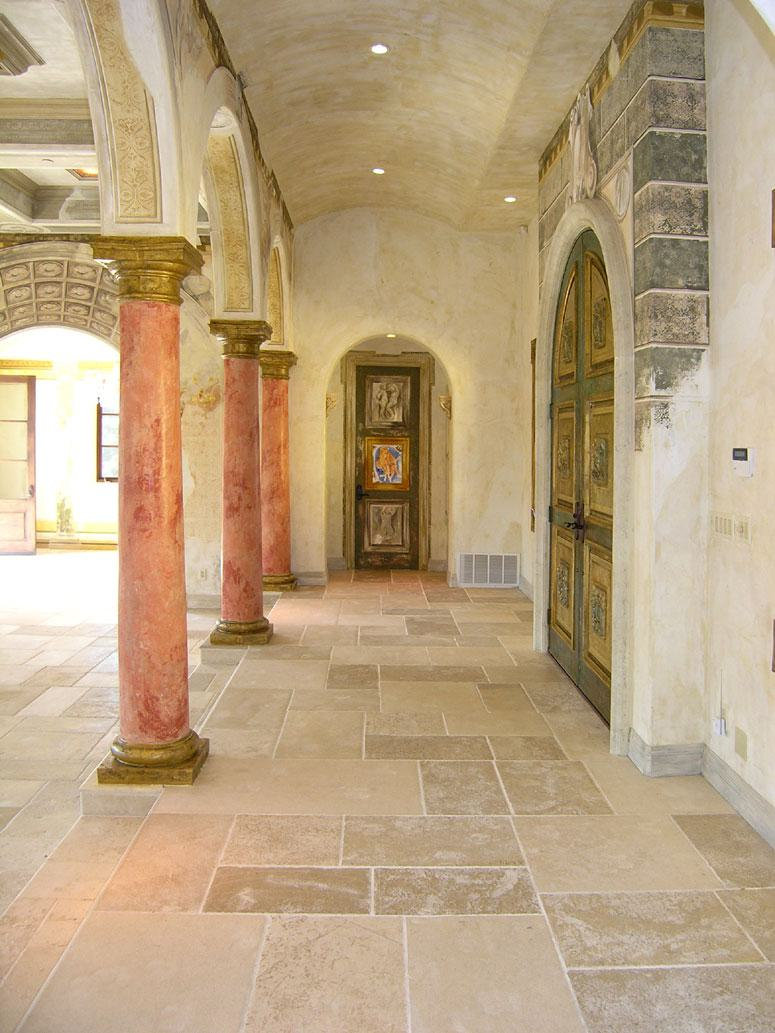
\includegraphics[width=0.12\textwidth,height=0.08\textwidth]{fig/castream/images/Outdataset/Corridor/Original/1L_10_Corridor_A.jpg}&
           \includegraphics[width=0.12\textwidth,height=0.08\textwidth]{fig/castream/images/Outdataset/Corridor/Attention/1L_10_Corridor_A.jpg}&
           \includegraphics[width=0.12\textwidth,height=0.08\textwidth]{fig/castream/images/Outdataset/Greenhouse/Original/20070417klpcnatun_229_Ies_SCO.jpg}&
           \includegraphics[width=0.12\textwidth,height=0.08\textwidth]{fig/castream/images/Outdataset/Greenhouse/Attention/20070417klpcnatun_229_Ies_SCO.jpg}&
           \includegraphics[width=0.12\textwidth,height=0.08\textwidth]{fig/castream/images/Outdataset/Poolinside/Original/141821195_M.jpg}&
           \includegraphics[width=0.12\textwidth,height=0.08\textwidth]{fig/castream/images/Outdataset/Poolinside/Attention/141821195_M.jpg}&
           \includegraphics[width=0.12\textwidth,height=0.08\textwidth]{fig/castream/images/Outdataset/WineCellar/Original/bodega_45_18_yahoo.jpg}&
           \includegraphics[width=0.12\textwidth,height=0.08\textwidth]{fig/castream/images/Outdataset/WineCellar/Attention/bodega_45_18_yahoo.jpg}\\
           
           \includegraphics[width=0.12\textwidth,height=0.08\textwidth]{fig/castream/images/Outdataset/Corridor/Original/430_Korridor_300.jpg}&
           \includegraphics[width=0.12\textwidth,height=0.08\textwidth]{fig/castream/images/Outdataset/Corridor/Attention/430_Korridor_300.jpg}&
           \includegraphics[width=0.12\textwidth,height=0.08\textwidth]{fig/castream/images/Outdataset/Greenhouse/Original/20070418klpcnaecl_364_Ies_SCO.jpg}&
           \includegraphics[width=0.12\textwidth,height=0.08\textwidth]{fig/castream/images/Outdataset/Greenhouse/Attention/20070418klpcnaecl_364_Ies_SCO.jpg}&
           \includegraphics[width=0.12\textwidth,height=0.08\textwidth]{fig/castream/images/Outdataset/Poolinside/Original/catalogue_piscine_interieur.jpg}&
           \includegraphics[width=0.12\textwidth,height=0.08\textwidth]{fig/castream/images/Outdataset/Poolinside/Attention/catalogue_piscine_interieur.jpg}&
           \includegraphics[width=0.12\textwidth,height=0.08\textwidth]{fig/castream/images/Outdataset/WineCellar/Original/bodega_63_24_flickr.jpg}&
           \includegraphics[width=0.12\textwidth,height=0.08\textwidth]{fig/castream/images/Outdataset/WineCellar/Attention/bodega_63_24_flickr.jpg}\\
           
           \includegraphics[width=0.12\textwidth,height=0.08\textwidth]{fig/castream/images/Outdataset/Corridor/Original/06_Right_corridor_of_the_main_hall.jpg}&
           \includegraphics[width=0.12\textwidth,height=0.08\textwidth]{fig/castream/images/Outdataset/Corridor/Attention/06_Right_corridor_of_the_main_hall.jpg}&
           \includegraphics[width=0.12\textwidth,height=0.08\textwidth]{fig/castream/images/Outdataset/Greenhouse/Original/2026_2006_Grimm_s_Gardens_Greenhouse.jpg}&
           \includegraphics[width=0.12\textwidth,height=0.08\textwidth]{fig/castream/images/Outdataset/Greenhouse/Attention/2026_2006_Grimm_s_Gardens_Greenhouse.jpg}&
           \includegraphics[width=0.12\textwidth,height=0.08\textwidth]{fig/castream/images/Outdataset/Poolinside/Original/connolly_center_pool_inside_lg.jpg}&
           \includegraphics[width=0.12\textwidth,height=0.08\textwidth]{fig/castream/images/Outdataset/Poolinside/Attention/connolly_center_pool_inside_lg.jpg}&
           \includegraphics[width=0.12\textwidth,height=0.08\textwidth]{fig/castream/images/Outdataset/WineCellar/Original/bodega_78_08_flickr.jpg}&
           \includegraphics[width=0.12\textwidth,height=0.08\textwidth]{fig/castream/images/Outdataset/WineCellar/Attention/bodega_78_08_flickr.jpg}\\              
    \end{tabular}
%    }
    \vspace{3pt}
    \caption{\textbf{Raw attention maps} obtained from our \Ours on images of the MIT 67 Scenes dataset \autocite{quattoni2009recognizing} on classes that do not exist in ImageNet. The network sees them at inference for the first time.} 
    %
    \label{fig:enter-label}
\end{figure}  
Indeed, the differences in saliency maps should not be large, as both methods share the same 
features maps $F^k_\ell$ and only the weight coefficients $\alpha^c_k$ differ.
Despite the small differences, the following quantitative results show that \Ours has a significant 
impact on the interpretability metrics.
   
In addition, \autoref{fig:enter-label} shows examples of images from the MIT 67 Scenes 
dataset \autocite{quattoni2009recognizing} along with raw attention maps obtained by \Ours. These 
images come from four classes that do not exist in ImageNet and the network sees them at inference for 
the first time. Nevertheless, the attention maps focus on objects of interest in general.

\newpage
\section{Quantitative Results}
\label{sec:ca_quant}

\newpage

